\section{Evaluation}
\label{sec:Evaluation}
For a complete listing of example results and a demonstration of UpvoteetovpU, please see the website at \url{http://www.cs.virginia.edu/~whh8b/upvoteetovpu/}. Also, to evaluate the source code, see the repository at \url{https://github.com/floydbe/Computer-Vision-Final-Project}.
\subsection{Strengths}
\label{sec:Strengths}
This algorithm performs exceptionally well under certain conditions. Thankfully, these conditions are not uncommon in real world videos. If the camera position is stable throughout a video, there is a higher chance for the distance between any pair of frames to be small. In this scenario, the differences in distances correspond strongly to ``interesting'' parts of the frames and background noise becomes less of an issue. Similarly, if there are no moving parts to the background, we obtain the same benefit. These conditions occur in many real videos, but are particularly common in animated videos. Consequently, the system performs well on those.

\subsection{Weaknesses}
\label{sec:Weaknesses}
\subsubsection{Masks}
\label{sec:MasksWeaknesses}

Because of the way that masks are calculated (either as the median or the mean of the pixel values throughout the video), some type of ``interesting'' movement may be classified as part of the background. Consider Figures~\ref{fig:mana} and \ref{fig:manb} which is a frame from a video of a man throwing a ball against a trampoline. The man's arms and the ball change position in almost every frame of the video. Because of this, it is easy for a median or average mask to isolate his arms and the ball. However, the man's torso (especially his upper legs) stay in almost exactly the same position throughout but constitute part of the interesting region in every frame of the video loop. This means that a median or average mask incorrectly classify those regions as part of the background. Figure x is a frame of a video where the a median mask has filtered out the background (by converting the pixels to black). It is easy to see that the man's legs are completely lost in the background. For these videos it is hard to apply masks in a coherent way. 
\begin{figure*}
\centering
\begin{minipage}{0.33\textwidth}
\centering
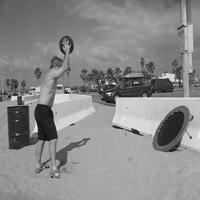
\includegraphics[width=2in]{frame_0074.jpg}
\caption{Still frame from video of man throwing ball.}
\label{fig:mana}
\end{minipage}\hfill
\begin{minipage}{0.33\textwidth}
\centering
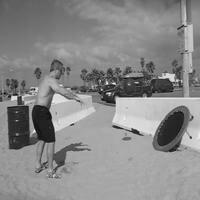
\includegraphics[width=2in]{frame_0076.jpg}
\caption{Still frame from video of man throwing ball.}
\label{fig:manb}
\end{minipage}
\begin{minipage}{0.33\textwidth}
\centering
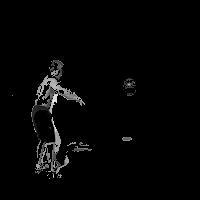
\includegraphics[width=2in]{median_man.jpg}
\caption{Still frame from video of median filter applied to video of man throwing ball.}
\end{minipage}
\end{figure*}

